\begin{frame}{Performance in Controllable Protein Generation}% on Four Different Instructions
	\begin{center}
		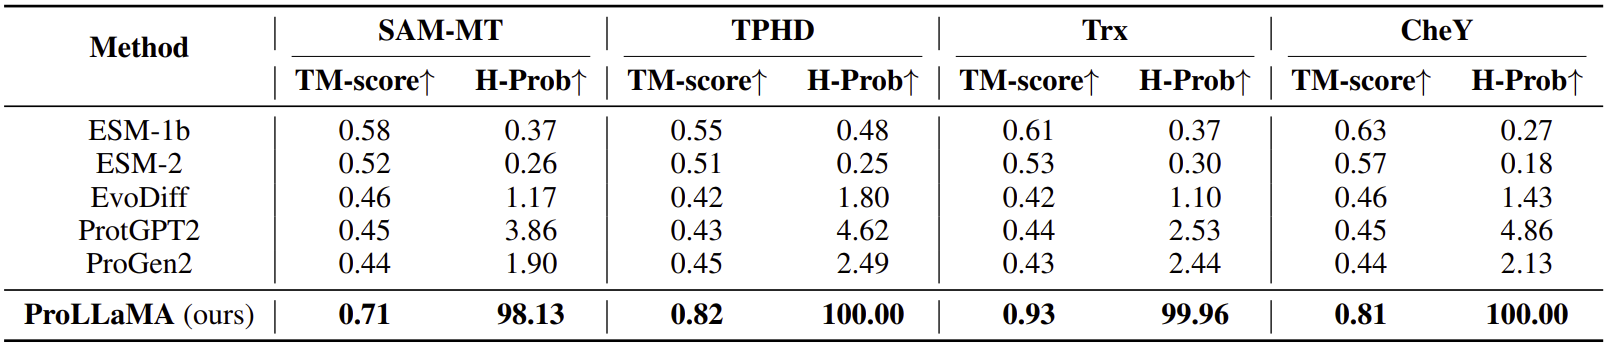
\includegraphics[scale=0.21]{tables/controlled_generation_comparison.png}
	\end{center}
	\vspace{-1em}\credit{Table}{lv2024prollama}
	\begin{itemize}
		\item ProLLaMA
		\begin{itemize}
			\item can generate protein sequences with desired functionalities
			\item Structures of generated proteins closely resemble those of natural proteins in the same superfamily, implying functional similarity.
			\item Generated proteins are homologous to natural ones and belong to the same superfamily.
		\end{itemize}
		\item Other models: much less controllable generation of proteins
		\item Superfamily descriptors: SAM-MT, TPHD, Trx, CheY
	\end{itemize}
\end{frame}